\section{Results and Analysis}

Same test program run linked to each (because portability).

\subsection{Data Movement in the Hash Table}

\begin{figure}
\centering
\hspace*{-0.3in}
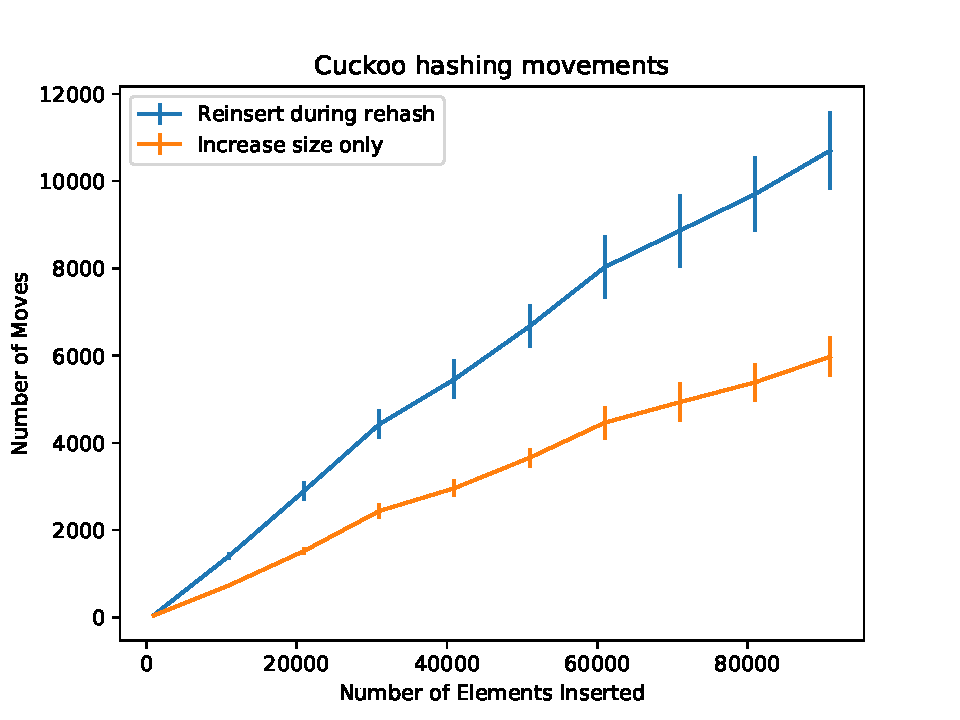
\includegraphics[width=85mm]{fig/moves}
\caption{Movement of buckets during insert for non-reinserting and standard
cuckoo hashing.}
\label{fig:moves}
\end{figure}

The overall number of moves done in the Cuckoo hashing implementation is shown
in Figure~\ref{fig:moves}, and shows that not reinserting elements produces a
significant reduction in the number of moves done during insert operations.
Since Cuckoo hashing is heavily dependent on hash function and workload, these
tests were performed by inserting elements with random keys and counting the
movements done in total, averaged over many runs with different seeds.
The comparison system is a nearly identical
implementation of Cuckoo hashing that reinserts all elements during a rehash.
The error bars show standard deviation, and demonstrate that the non-reinserting
rehashing strategy is less dependent on workload and hash function than standard
cuckoo hashing.

\subsection{Performance}

\begin{figure}
\centering
\hspace*{-0.5in}
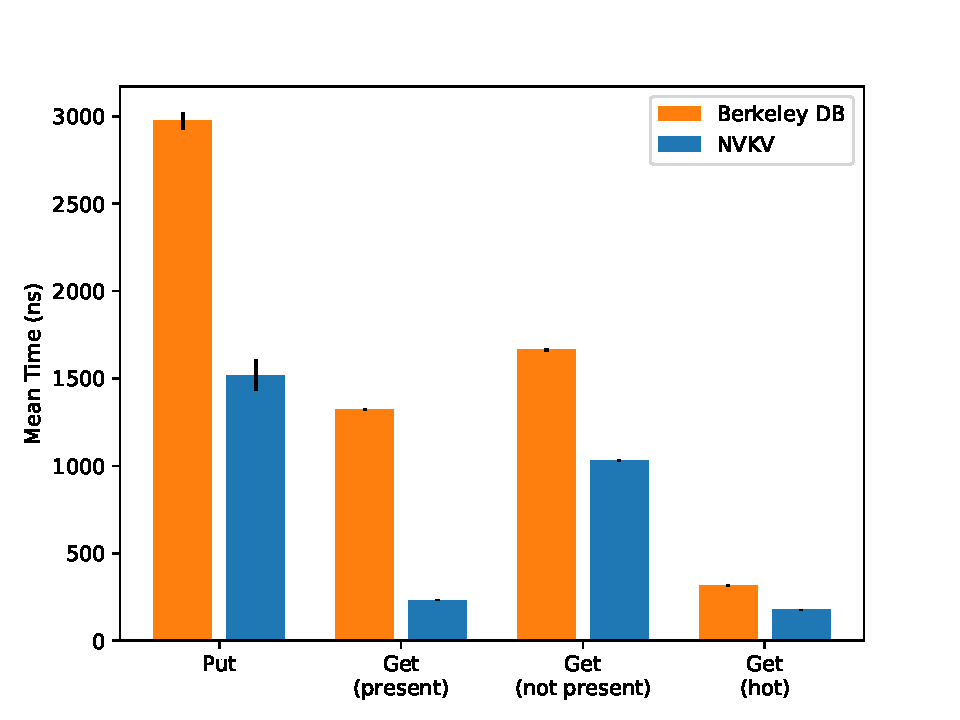
\includegraphics[width=98mm]{fig/perf}
\caption{Latency of various operations for both Berkeley DB and NVKV.}
\label{fig:perf}
\end{figure}

The average latency of insert and lookup operations is shown in
Figure~\ref{fig:perf}. The operations tested are \texttt{put}, which inserts an
element is not present, \texttt{get (present)}, which
looks up an element that is in the database, \texttt{get (not present)}, which
looks up an element that is \textit{not} in the database, and \texttt{get
(hot)}, which looks up the same element repeatedly. The error bars indicate
standard deviation, and are very tight due to the number of tests which were run
on each system. The latency of NVKV operations are significantly lower than the
equivalent Berkeley DB operations due to not needing any system calls in order
to ensure the required consistency and persistence of the insert operations.
Note, however, that the latency of \texttt{put} and \texttt{get (not present)}
is still high for NVKV. In the case of \texttt{put}, this is because of the
overhead of the transactional begin and commit statements along with the
persist-release operations required during the data recording phase of the
insert. In the case of \texttt{get (not present)}, the extra latency comes from
needing to search the hash table at each level that the element \textit{could}
be present.







\begin{figure}
\centering
\hspace*{-0.2in}
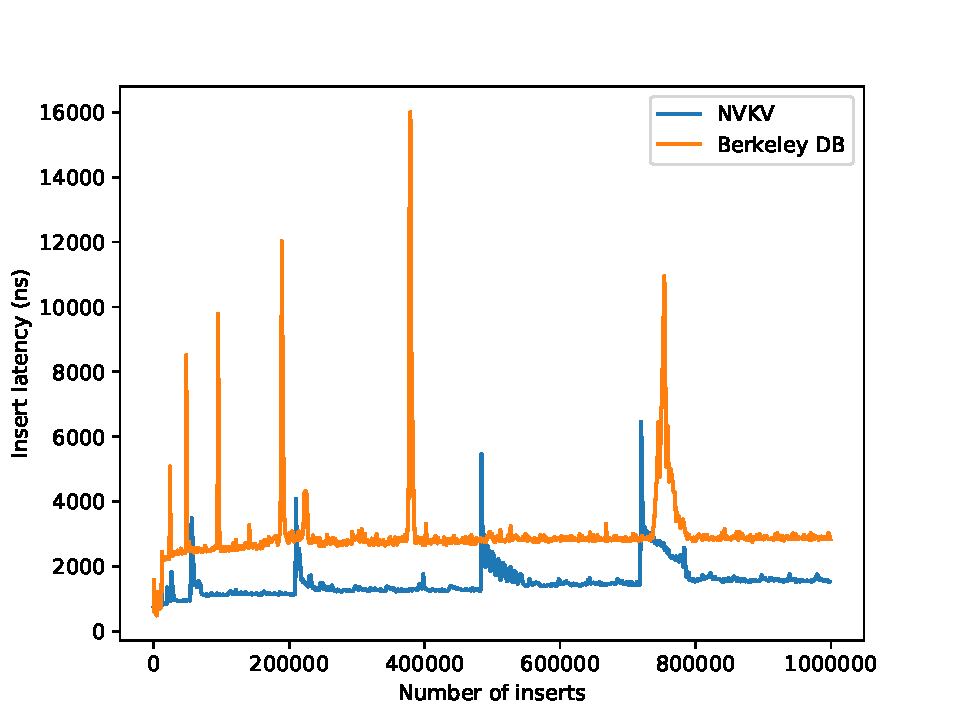
\includegraphics[width=94mm]{fig/line}
\caption{Insert performance as database size grows for both Berkeley DB and
NVKV.}
\label{fig:line}
\end{figure}

Figure~\ref{fig:line} shows the insert performance as a function of the number
of elements in the database for both Berkeley DB and NVKV. As is consistent with
Figure~\ref{fig:perf}, the average insert latency of NVKV is less than Berkeley
DB. Both have significant spikes which are caused by some rearrangement
procedure (in the case of NVKV these correspond to the hash table expansion
procedure).  Note that the NVKV spikes are much smaller, likely due to the
relatively cheap rehashing procedure that does not require reinserting elements.
The NVKV spikes also have a tail to the right of them where the latency remains
significantly above the mean for a time following a hash table expansion. I
expect that this is because the hash table is extremely unbalanced after the
table expansion, resulting in a large number of collisions and movements for
some time after the table is expanded. However, since the elements are always
reinserted at the top level, eventually these collisions will automatically
balance the table as more elements are inserted, amortizing the work of
reinserting during a rehash over future inserts.



